\chapter{GradCAM}

One of the most proeminent model-specific methods to acquire explanations for classification with CNNs is GradCAM. The intuition for the method is simple. At the last conovlutional layers, we have several channels that represent each a different feature. Those features are used by the next part of the network to produce the final output. If we want to know which parts of the image are being more useful to the network, we can look at the feature maps and observe which parts of the image are generating the signal used by the rest of the network. 

The problem with this approach is that the features have informations about all the output classes. How we know what features are more important to the decision? The idea behind GradCAM is to \textbf{average the feature maps weighted by the gradient} of each channel with respect to a specific class. 

However, this will still highlight the regions that have a negative influence to the decision. To filter out those regions, the result is passed through ReLU. The result is a coarse heatmap of the image highlighting important regions.

The formula for the heatmap with regard to the class $c$ is:

\begin{equation}
    H  = \text{ReLU}(\sum_k \alpha_k^c A^k)
    \label{eq:heatmap}
\end{equation}

Where $\alpha_k^c$, the weight of the $k$-th feature map for the class $c$, is defined as:

\begin{equation}
    \alpha_k^c=\frac{1}{Z} \sum_i \sum_j \frac{\partial y^c}{\partial A^k_ij}
    \label{eq:alpha}
\end{equation}

Where $A^k$ is the $k$-th feature map, $y^c$ is the output for the $c$ class, and $Z$ is the number of neurons in each map.

To visualize the process, we will use the ResNet-18 \cite{resnet} trained on the ImageNet dataset, with the weights available at PyTorch. We will use as input two images of airplanes.

\begin{figure}
    \centering
    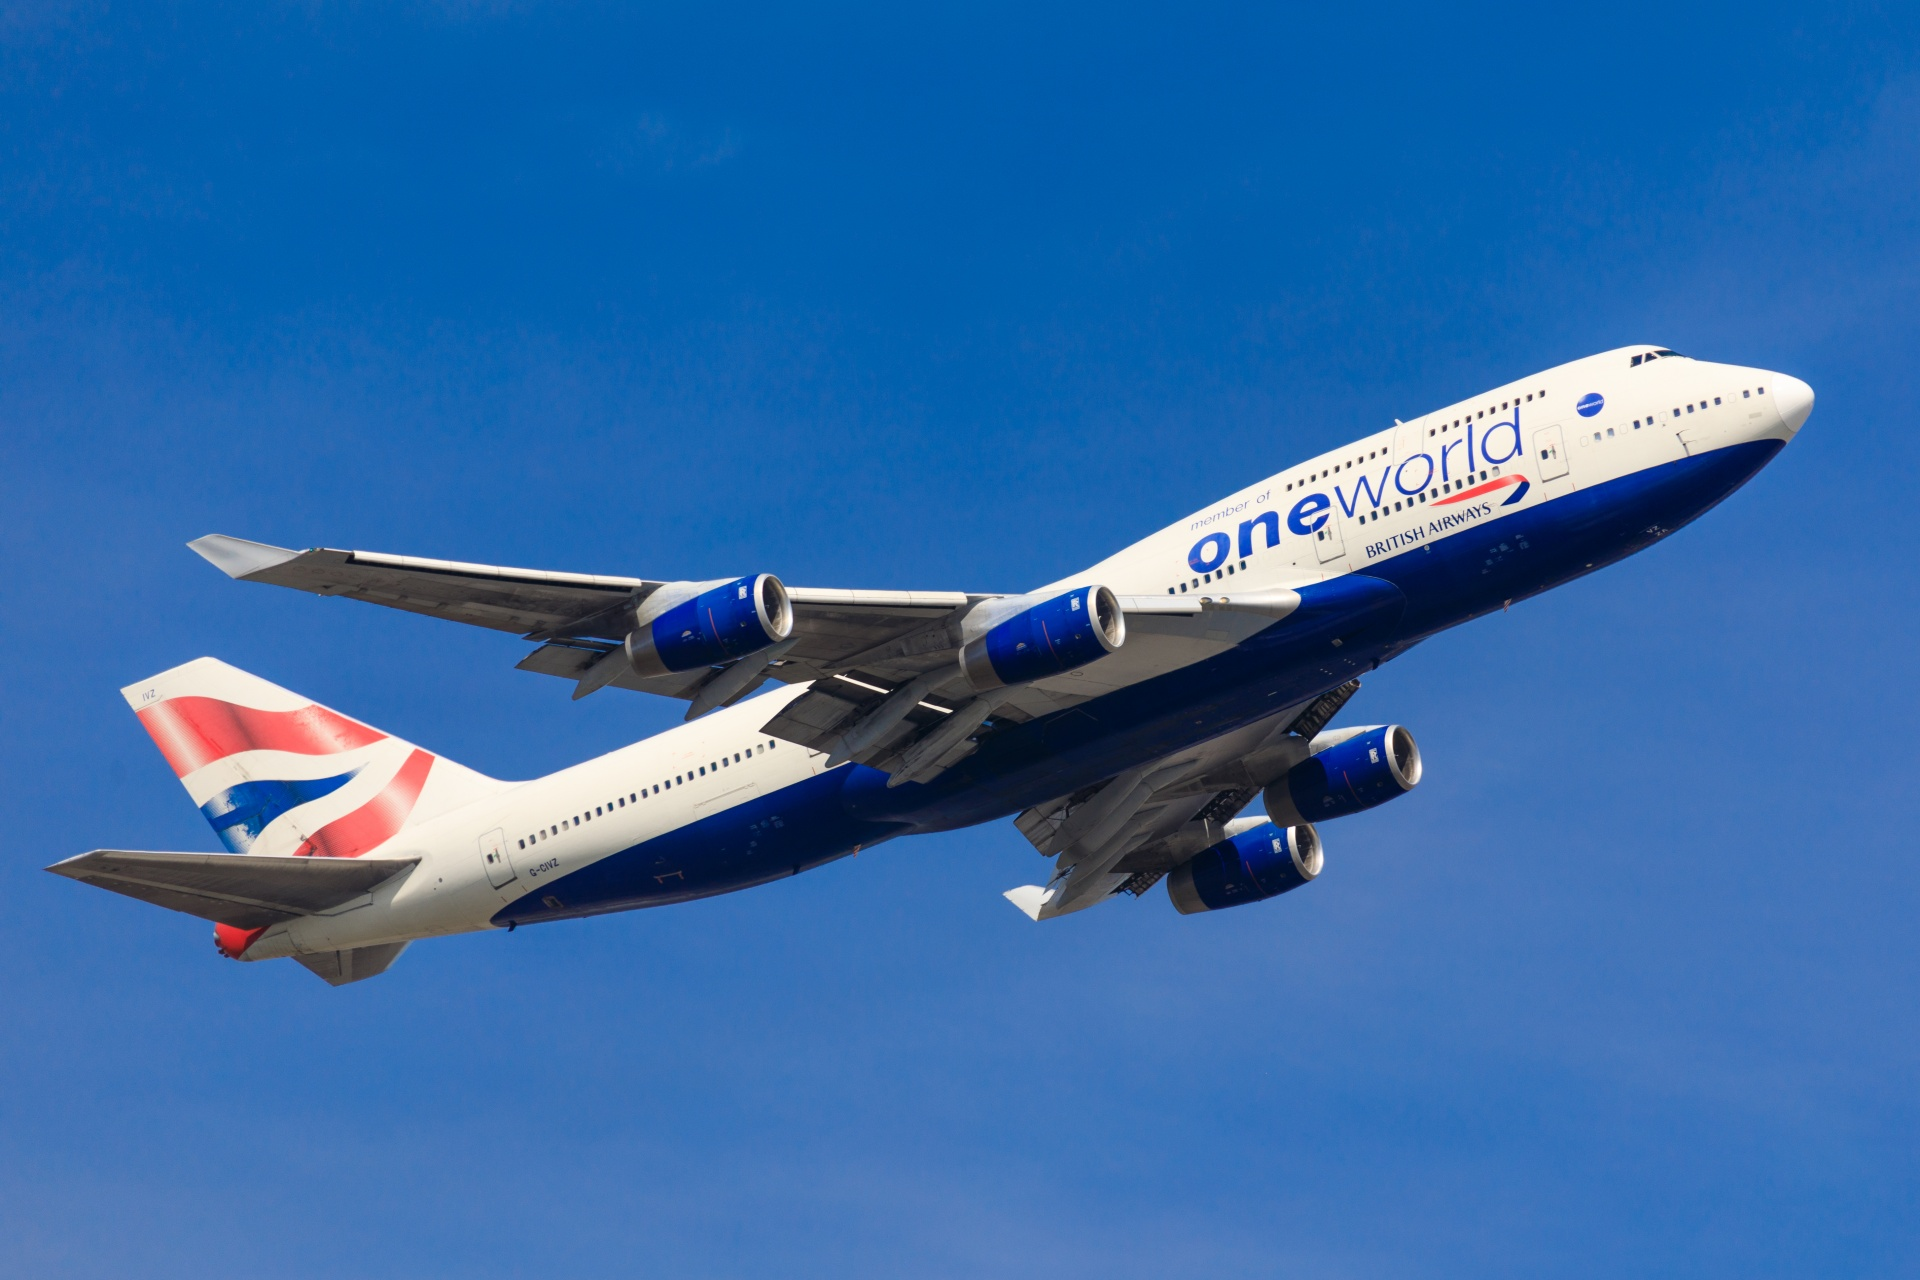
\includegraphics[width=0.4\linewidth]{gradcam/aviao2}
    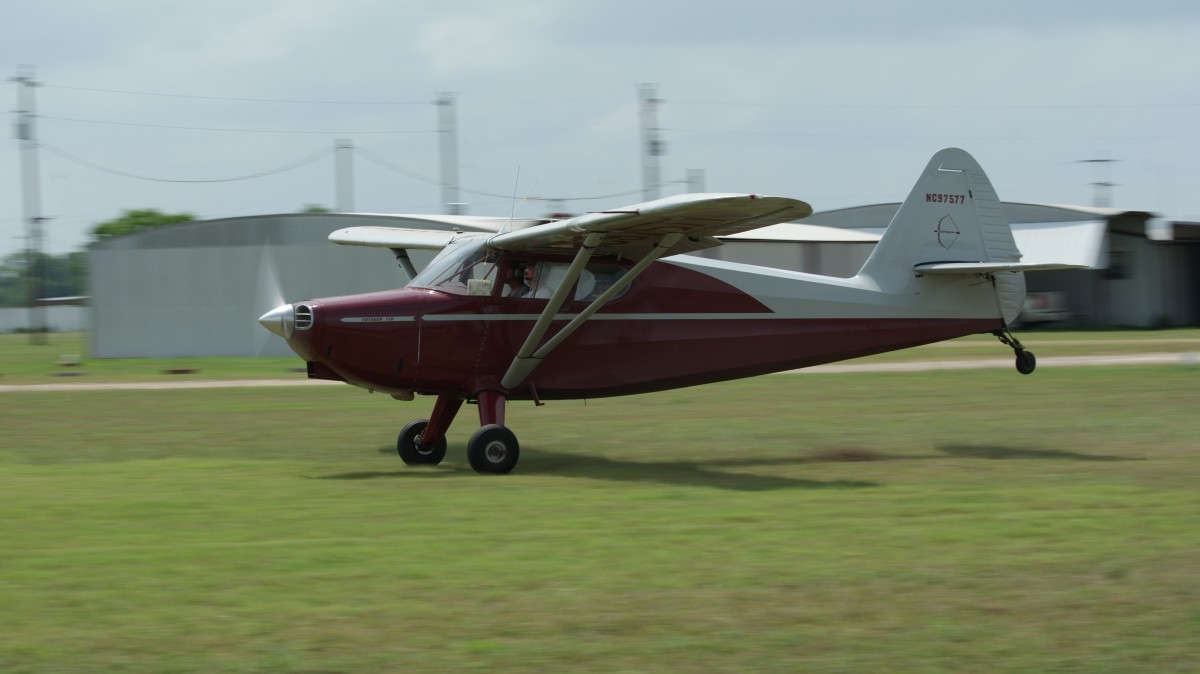
\includegraphics[width=0.4\linewidth]{gradcam/aviao3}
    \caption{Input images}
\end{figure}

The first step is to store the activations of the last convolutional layer of the network for each of the images. For this network, we have 512 channels at the last layer.


\begin{figure}
    \centering
    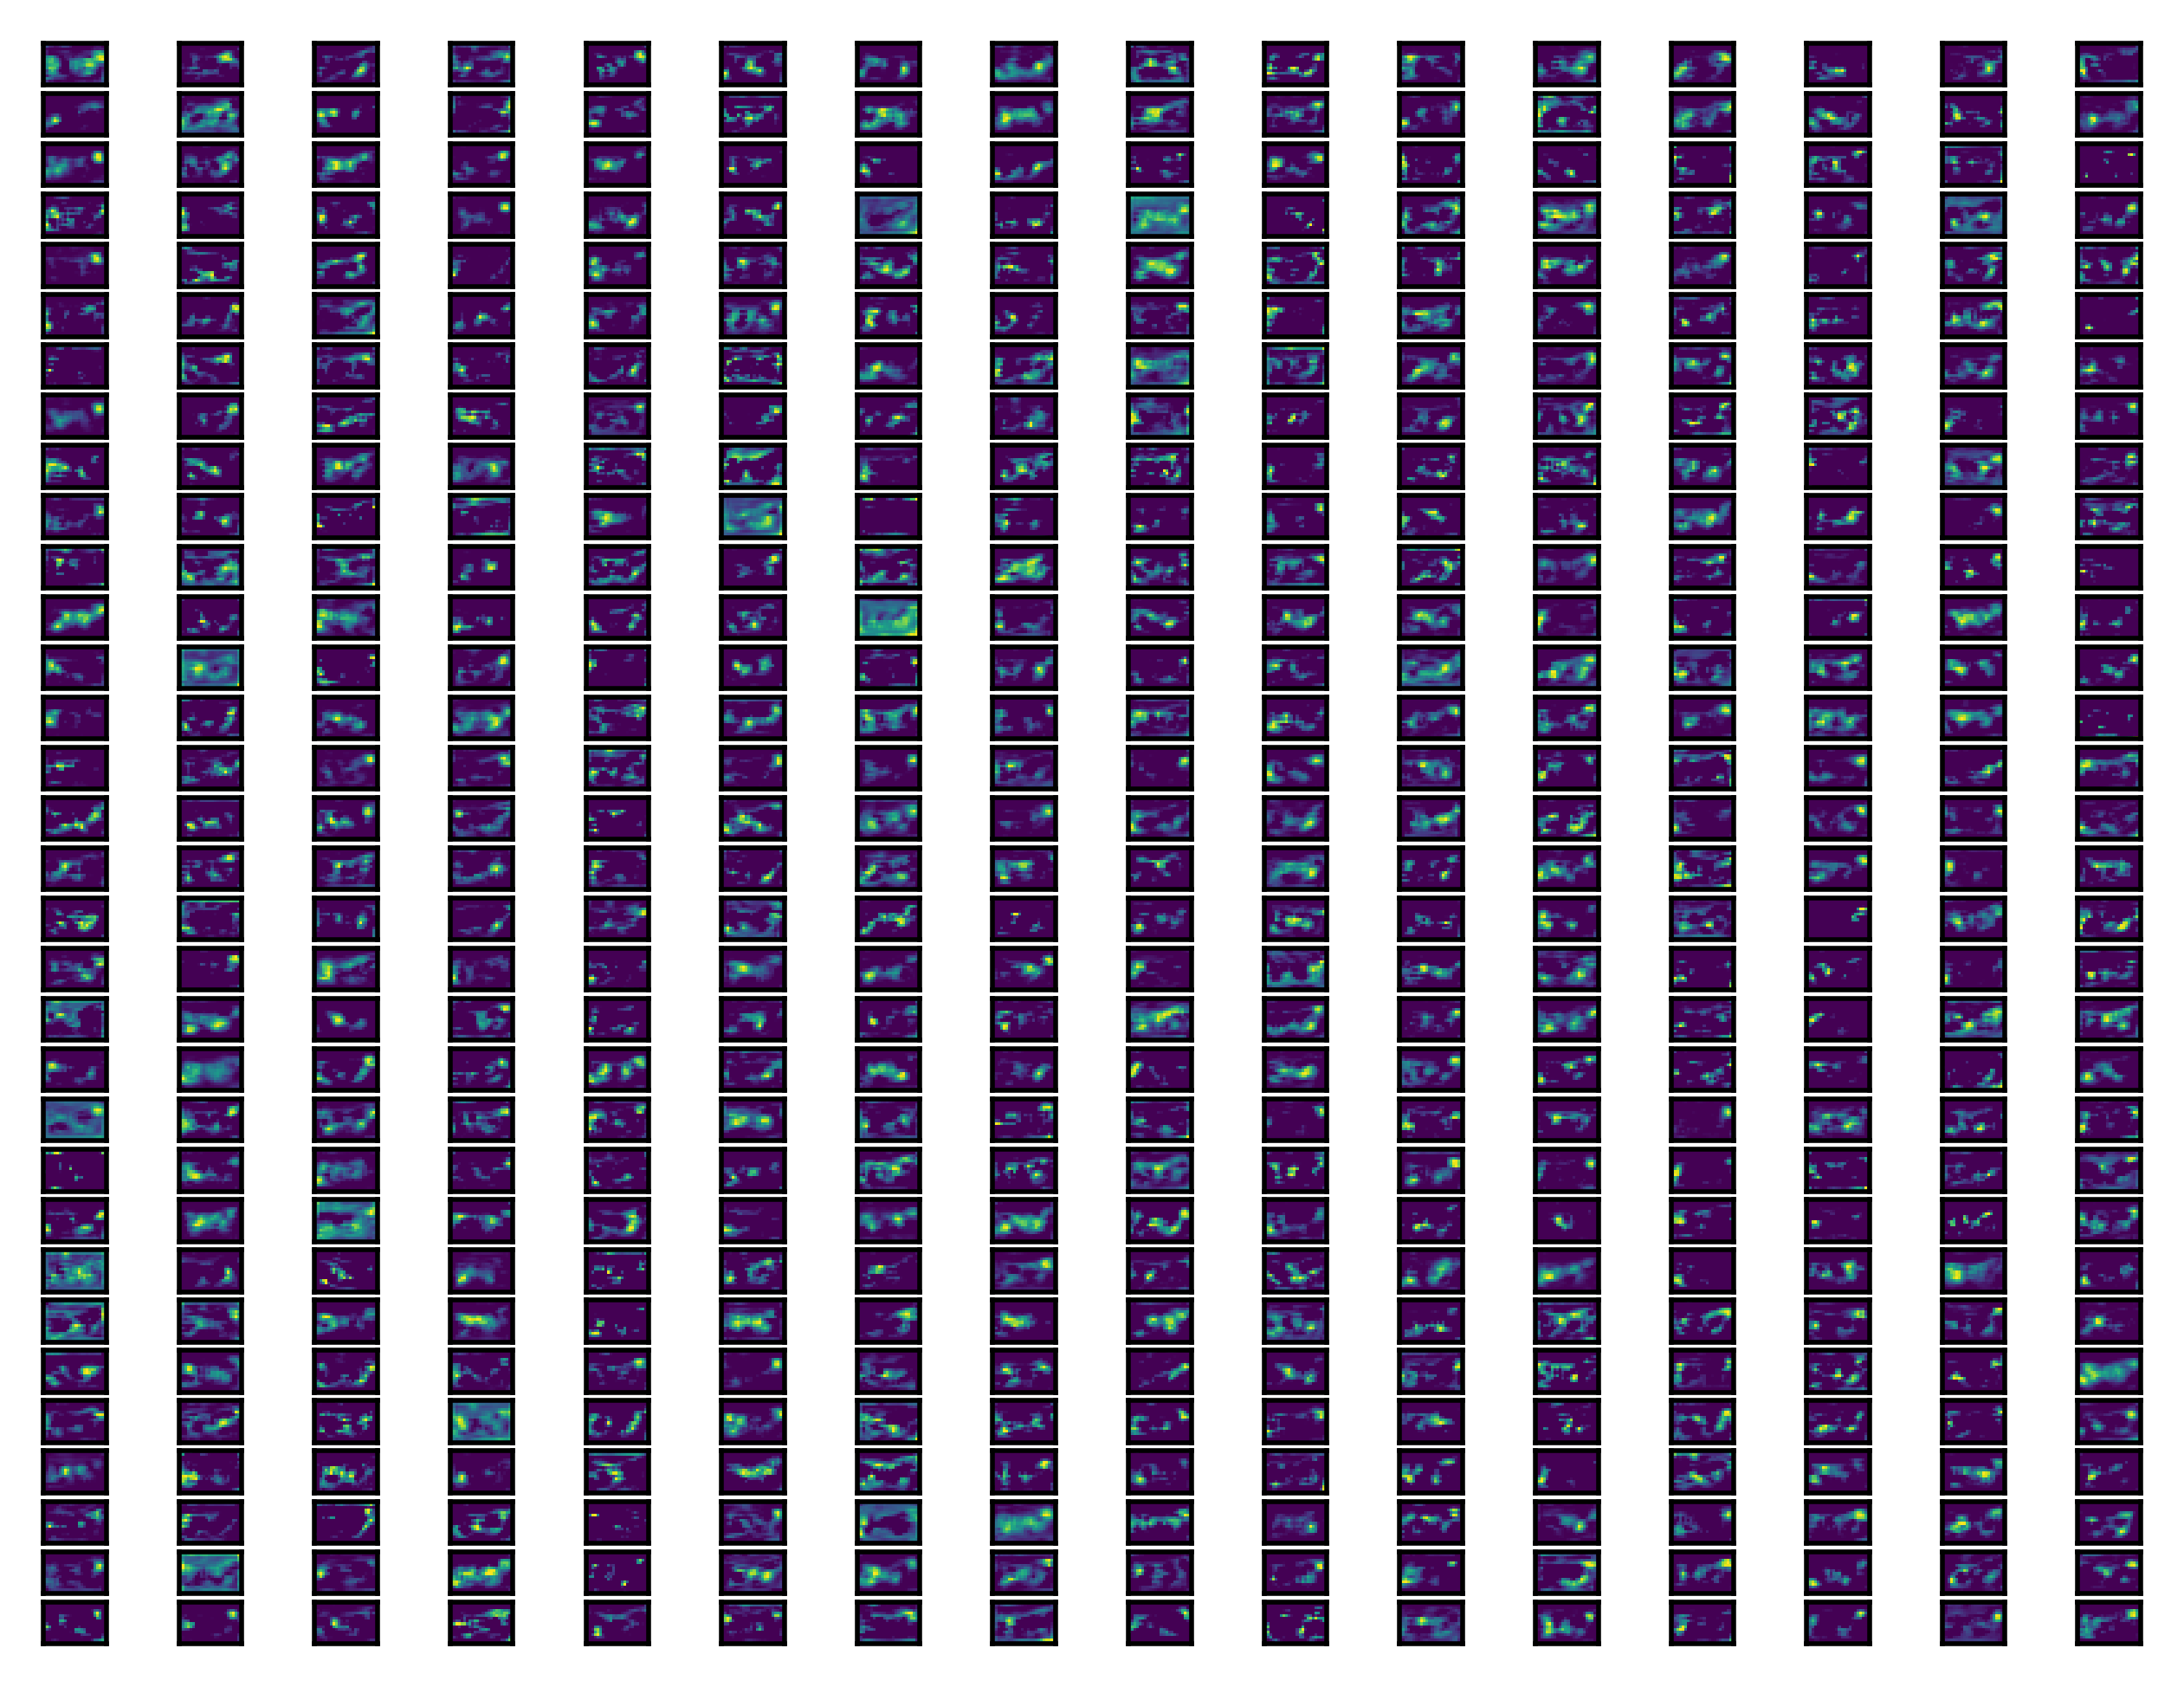
\includegraphics[width=0.4\linewidth]{gradcam/aviao2_activations}
    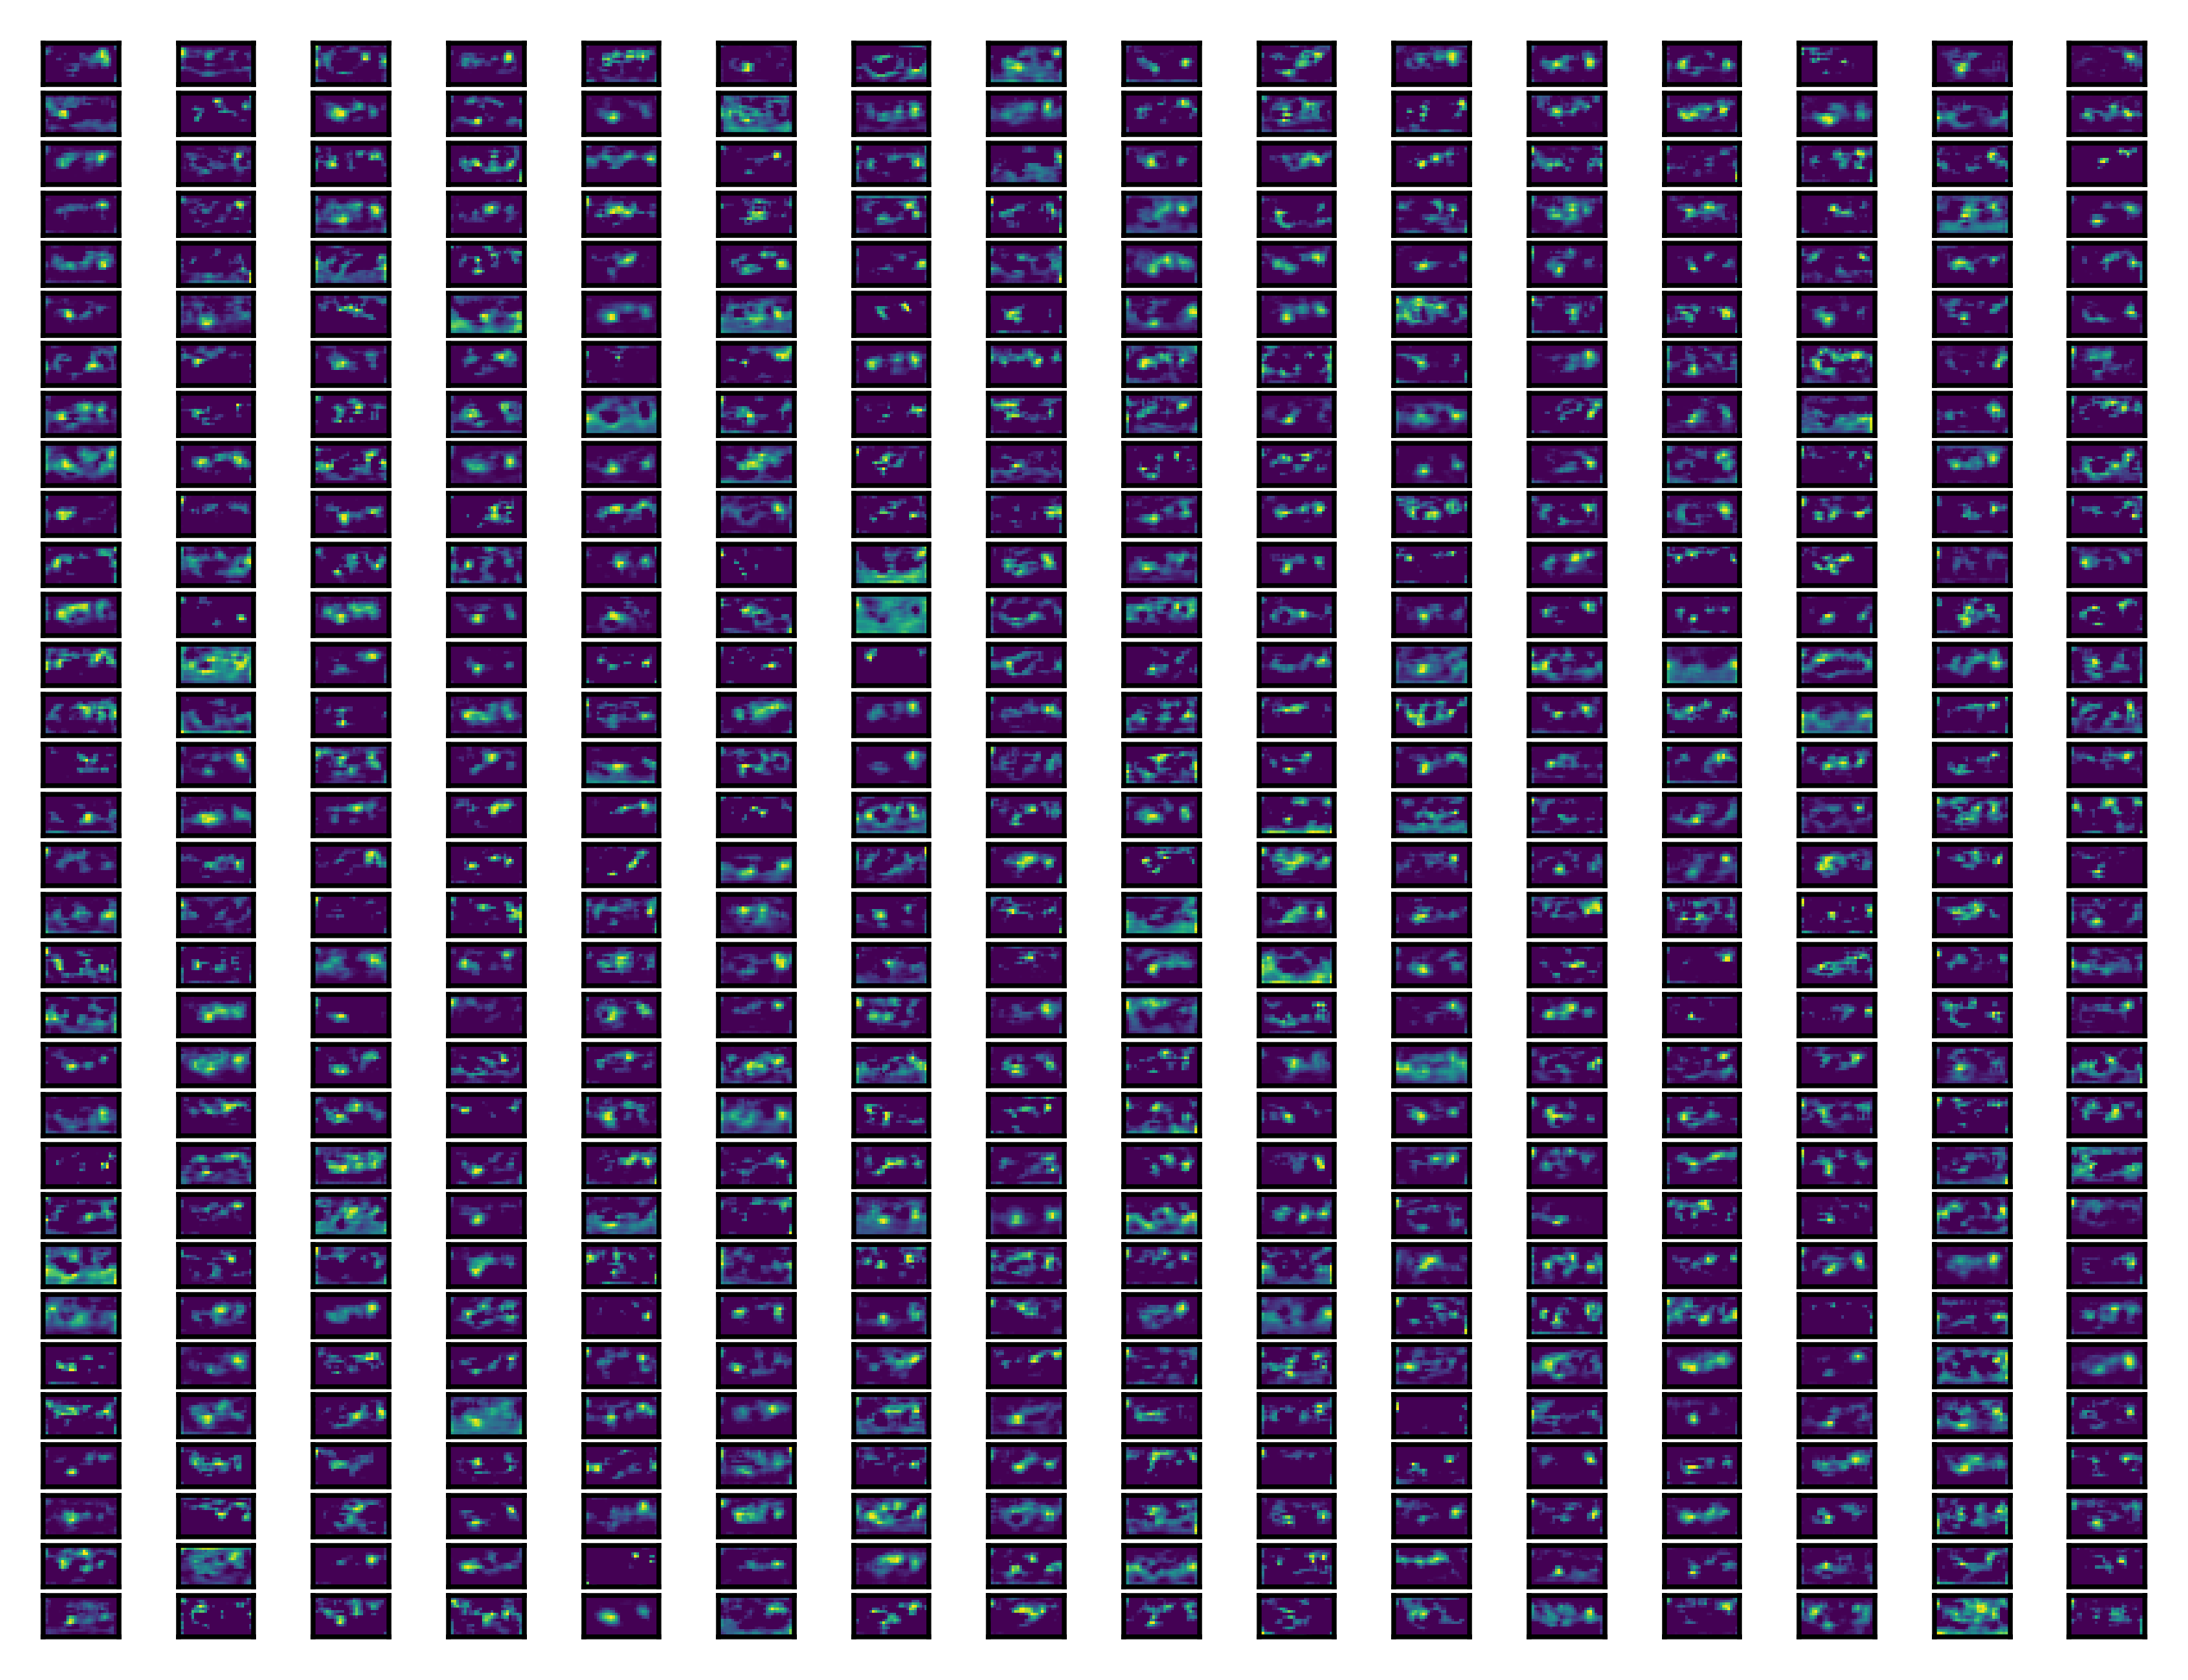
\includegraphics[width=0.4\linewidth]{gradcam/aviao3_activations}
    \caption{Activations of last convolutional layer}
    \label{fig:activations}
\end{figure}

The next step is to calculate the weight of each channel, according to \cite{eq:alpha}. We can then visualize the weights as a heatmap (each vertical line represents a channel):

\begin{figure}
    \centering
    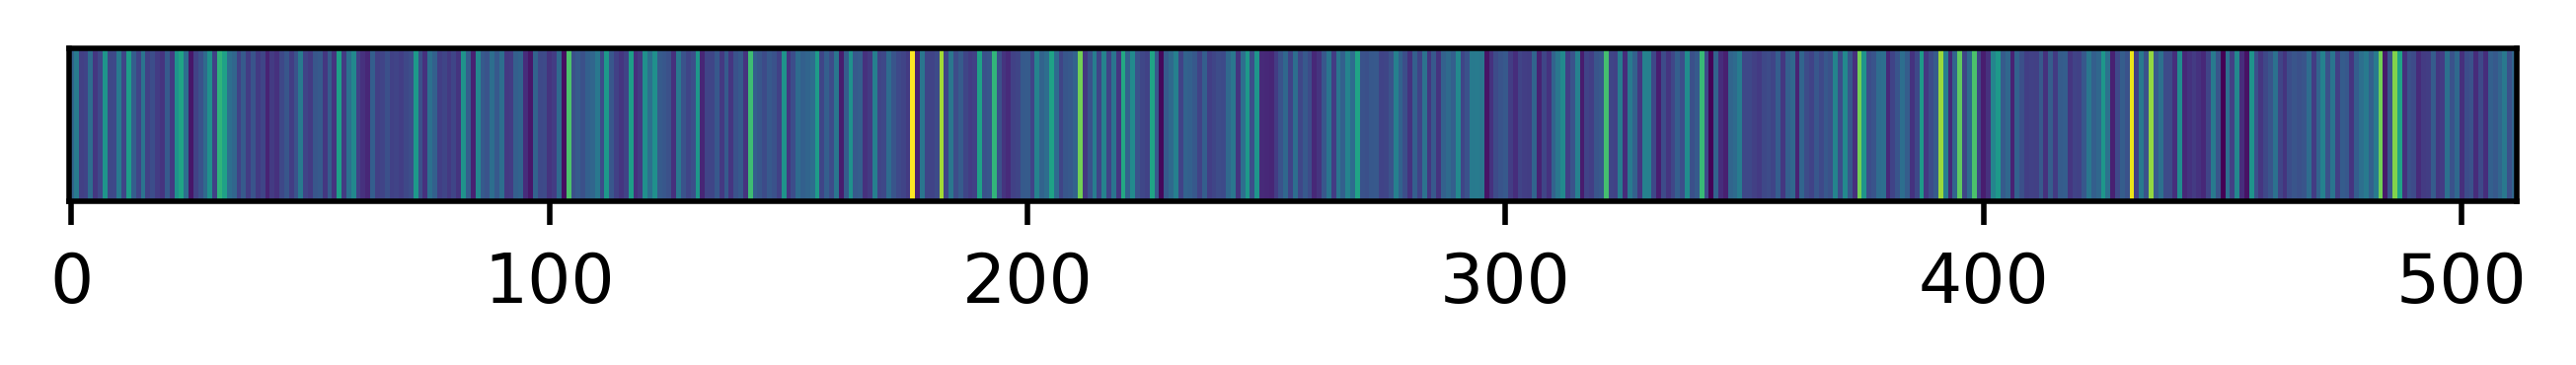
\includegraphics[width=0.4\linewidth]{gradcam/aviao2_alphas}
    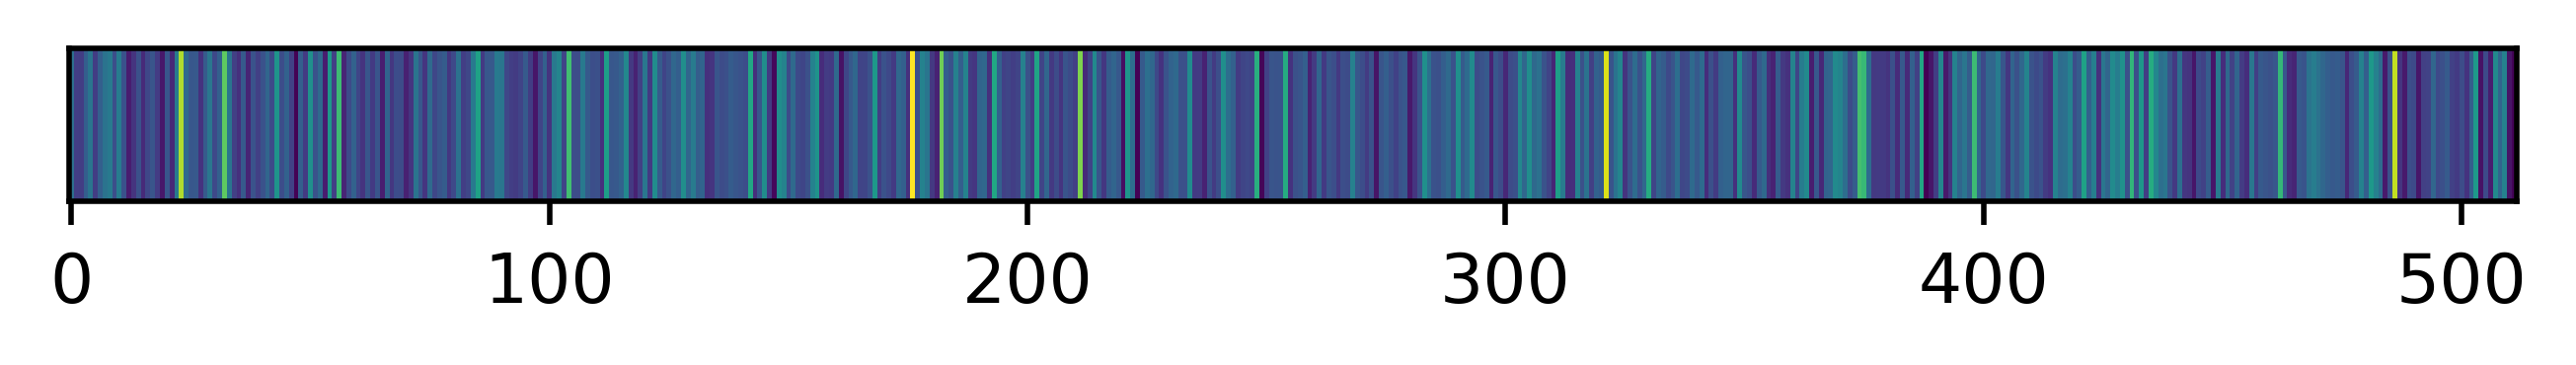
\includegraphics[width=0.4\linewidth]{gradcam/aviao3_alphas}
    \caption{Weight of each channel of the last convolutional layer}
    \label{fig:weights}
\end{figure}

By calculating the average of the activations found at \cite{fig:actiovations} weighted by \label{fig:weights}, we can achieve a heatmap highlighting important regions of each image:

\begin{figure}[H]
    \centering
    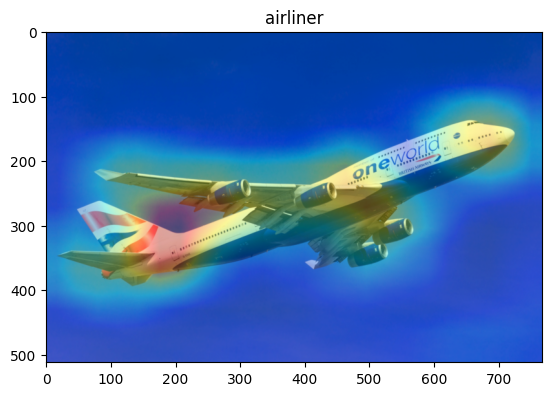
\includegraphics[width=0.4\linewidth]{gradcam/aviao2-GC}
    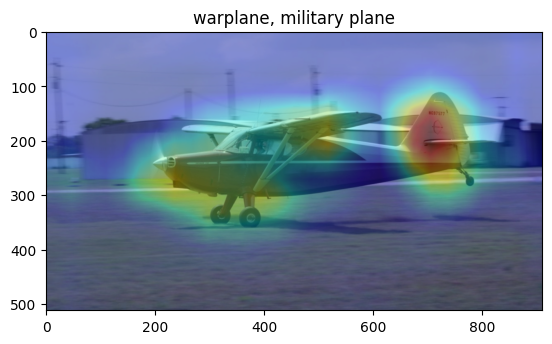
\includegraphics[width=0.4\linewidth]{gradcam/aviao3-GC}
    \caption{Result of GradCAM}
\end{figure}


\section{Guided Backpropagation}

Guided Backprogation is one of the most proeminent way of creating saliency maps. Following the same idea behind the application of the ReLU function at \cite{eq:heatmap}, we filter out negative gradients through the network, allowing the visualization of only positive influences.

\begin{figure}
    \centering
    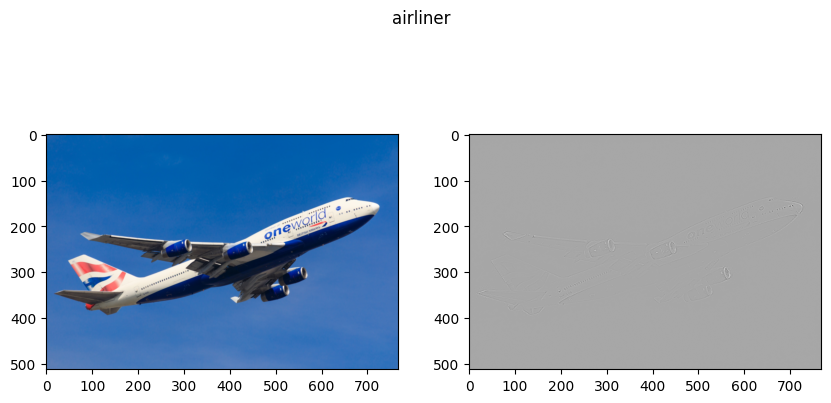
\includegraphics[width=0.8\linewidth]{gradcam/aviao2-GB}    
    \caption{Results of Guided Backpropation}
\end{figure}

\begin{figure}
    \centering
    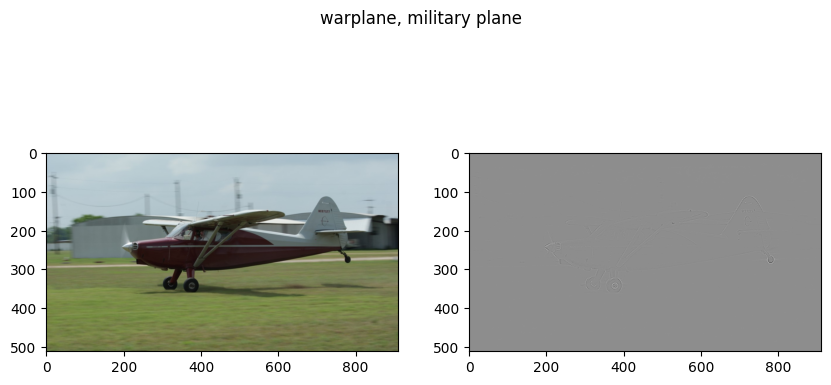
\includegraphics[width=0.8\linewidth]{gradcam/aviao3-GB}    
    \caption{Results of Guided Backpropation}
\end{figure}

\section{Guided GradCAM}

The output of GradCAM has the dimensions of the last convolutional layer of the network, and has to be upsampled to be overlayed on top of the input image. This results in a very coarse heatmap, with rough borders and lost details. To solve this, we can multiply (pixel by pixel) the heatmap with other simpler method, as guided-backpropagation. 

\begin{figure}
    \centering
    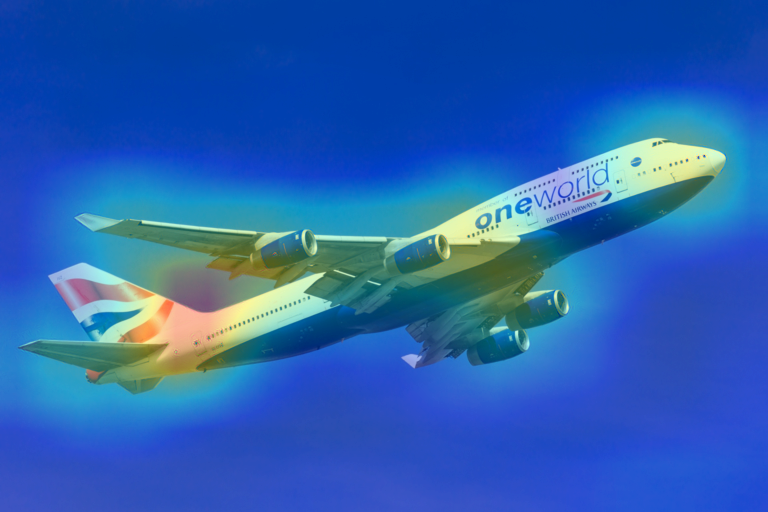
\includegraphics[width=0.4\linewidth]{gradcam/aviao2-GGC_RAW}
    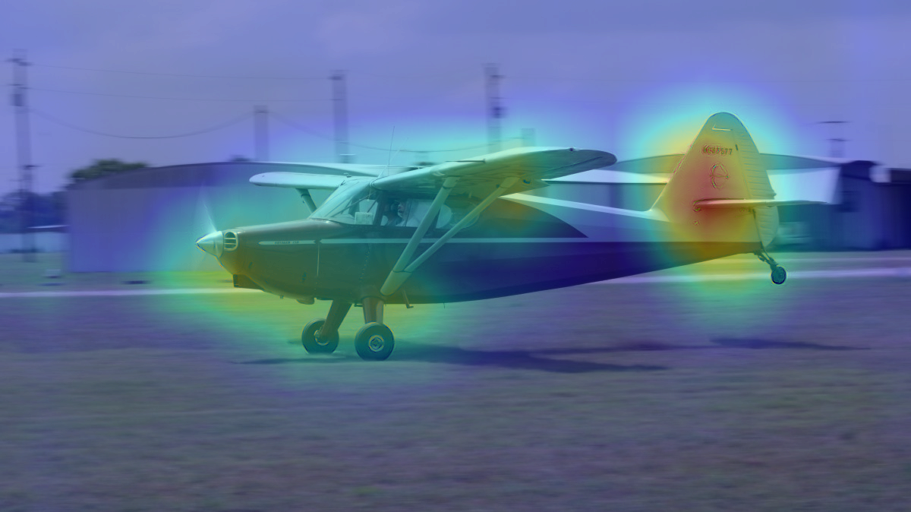
\includegraphics[width=0.4\linewidth]{gradcam/aviao3-GGC_RAW}
    \caption{Results of Guided GradCAM}
\end{figure}


\section{Implementation}

All these images were generated using the Python library \href{https://pytorch.org/}{Pytorch}. The implementation used a feature of the library called hooks. Hooks are functions that can be connected to the network. Those hooks will be called either at the forward pass (for forward hooks), or at the backward pass (for backward hooks). We used those hooks to register the activations and the gradient at GradCAM, and to filter out negative gradients at Guided Backpropagation.
\begin{program}
    \index{Python}
    \centering
    \label{code:gradcam_class}
    \begin{lstlisting}[language=Python, style=wider]
        class GradCAM:

        def __init__(self, model):
          self.activations=None
          self.gradients=None
          self.model=model
          self.model.eval()
          def forward_hook(module, input, output):
            self.activations = output
      
          def backward_hook(module, input, output):
            self.gradients = output[0]
      
      
          model._modules['layer4'].register_forward_hook(forward_hook)
          model._modules['layer4'].register_backward_hook(backward_hook)
      
      
        def forward(self, im):
          self.model.zero_grad()
          output = self.model(im)
          label = output.argmax().item()
          output[0,label].backward()
          alpha = self.gradients.squeeze(0).mean(dim=(1, 2))
          print(categories_MNIST[label])
          heatmap =  (self.activations.squeeze(0) * alpha.view(-1, 1, 1)).sum(dim=0)
          heatmap = transforms.Resize(im.shape[2:])(heatmap.unsqueeze(0))/heatmap.max()
          return (torch.clamp(heatmap, min=0).cpu(), categories_MNIST[label])
      
      
      
    \end{lstlisting}

    \caption{GradCAM Class}

    
\end{program}

\begin{program}
    \index{Python}
    \centering
    \label{code:gbp_class}
    \begin{lstlisting}[language=Python, style=wider]
        

class GuidedBackPropagation:
  def __init__(self, model):
    self.activations=None
    self.gradients=None
    self.model=model
    self.model.eval()

    def backward_hook(module, input, output):
      if isinstance(module, torch.nn.ReLU):
        return (torch.clamp(input[0], min=0),)



    for i, module in enumerate(model.modules()):
      if isinstance(module, torch.nn.ReLU):
        module.inplace = False
        module.register_full_backward_hook(backward_hook)


  def forward(self, im):
    self.model.zero_grad()
    output = self.model(im)
    label = output.argmax().item()
    print(label)
    output[0,label].backward()
    ret = im.grad.clone()
    ret = ret.squeeze(0).sum(0)
    ret = (ret - ret.min())/(ret.max() - ret.min())
    return (ret.cpu(), categories_MNIST[label])

    
    \end{lstlisting}

    \caption{GradCAM Class}

    
\end{program}

Following is an example of the utilization of those classes:

\begin{program}
    \index{Python}
    \centering
    \label{code:using_gc_gbp}
    \begin{lstlisting}[language=Python, style=wider]
from util import *
from GradCam import *
from glob import glob

model = torchvision.models.resnet18(weights=torchvision.models.ResNet18_Weights.IMAGENET1K_V1).to(device).eval()
inp_trans = transforms.Compose([transforms.Resize(512), transforms.ToTensor(), transforms.Normalize(mean=[0.485, 0.456, 0.406], std=[0.229, 0.224, 0.225]),])
view_trans=transforms.Compose([transforms.Resize(512), transforms.ToTensor()])


files=glob('./imagens/*')
images=[Image.open(f) for f in files]
tensors = [inp_trans(im).unsqueeze(0).to(device) for im in images]
view_tensors = [view_trans(im).unsqueeze(0).to(device) for im in images]
print(len(tensors))

gr = GradCAM(model)
heatmaps=[gr.forward(tensor) for tensor in tensors]

gb = GuidedBackPropagation(model)
bp = [gb.forward(tensor.requires_grad_()) for tensor in tensors]

      
    \end{lstlisting}

    \caption{Utilization of the classes}

    
\end{program}

